\newpage
\section{Database design}

\subsubsection{Description}
The Enhanced Entity--Relationship Diagram (EERD) describes the conceptual data model of the proposed system, highlighting how users, physical devices, and monitored environments are connected within a unified platform. At the core of the model are three principal entities: \textbf{User}, \textbf{Devices}, and \textbf{Environments}. These entities represent the main human actors, the physical components deployed in the system, and the operational spaces in which monitoring and interaction take place.

The \textbf{User} entity represents individuals who access and interact with the system. A user can initiate multiple \textbf{Interaction Sessions}, which capture the communication context between the user and the platform. Each interaction session stores information such as the input text, start date, and latest update time, allowing the system to track user requests over time. In addition, each session is associated with a specific \textbf{AI Model}, indicating which intelligent model is used to process the interaction. This relationship enables the system to support AI-assisted monitoring and response generation while maintaining traceability of the model involved in each session.

The \textbf{Environments} entity represents the physical or logical spaces where system operations occur. An environment can correspond to a monitored room, building area, or deployment context. It serves as an important organizational unit because both user interactions and device activities are tied to a specific environment. Within each environment, multiple \textbf{Devices} can be deployed, reflecting the one-to-many relationship between operational spaces and IoT components.

The \textbf{Devices} entity models the hardware units operating in the system, such as sensors or other monitoring equipment. Each device is characterized by its name, category, status, and anomaly score, which help represent its identity, function, operational state, and analytical condition. Devices play an important role in system monitoring because they generate both telemetry data and activity records. Through this design, the system can monitor device behavior while also linking device outputs to the broader environmental and user-interaction context.

To support monitoring functions, the model includes \textbf{Telemetry Points}, which store time-based sensor measurements such as temperature, humidity, and recorded timestamps. These telemetry records are produced within environments and are associated with devices, allowing the system to capture real-time environmental conditions and trace them back to their originating hardware sources. Alongside telemetry data, \textbf{Activity Logs} record notable events generated during system operation. These logs are related to users, interaction sessions, environments, and devices, thereby providing a structured audit trail for analysis, diagnostics, and system transparency.

Overall, the EERD provides a coherent conceptual foundation for the system by integrating user interaction, AI-supported processing, environmental monitoring, device management, and event logging into a single database structure. This design supports both operational management and future analytical extensions, making it suitable for intelligent monitoring applications.

\subsection{Enhanced Entity--Relationship Diagram}

\begin{figure}[H]
	\centering
	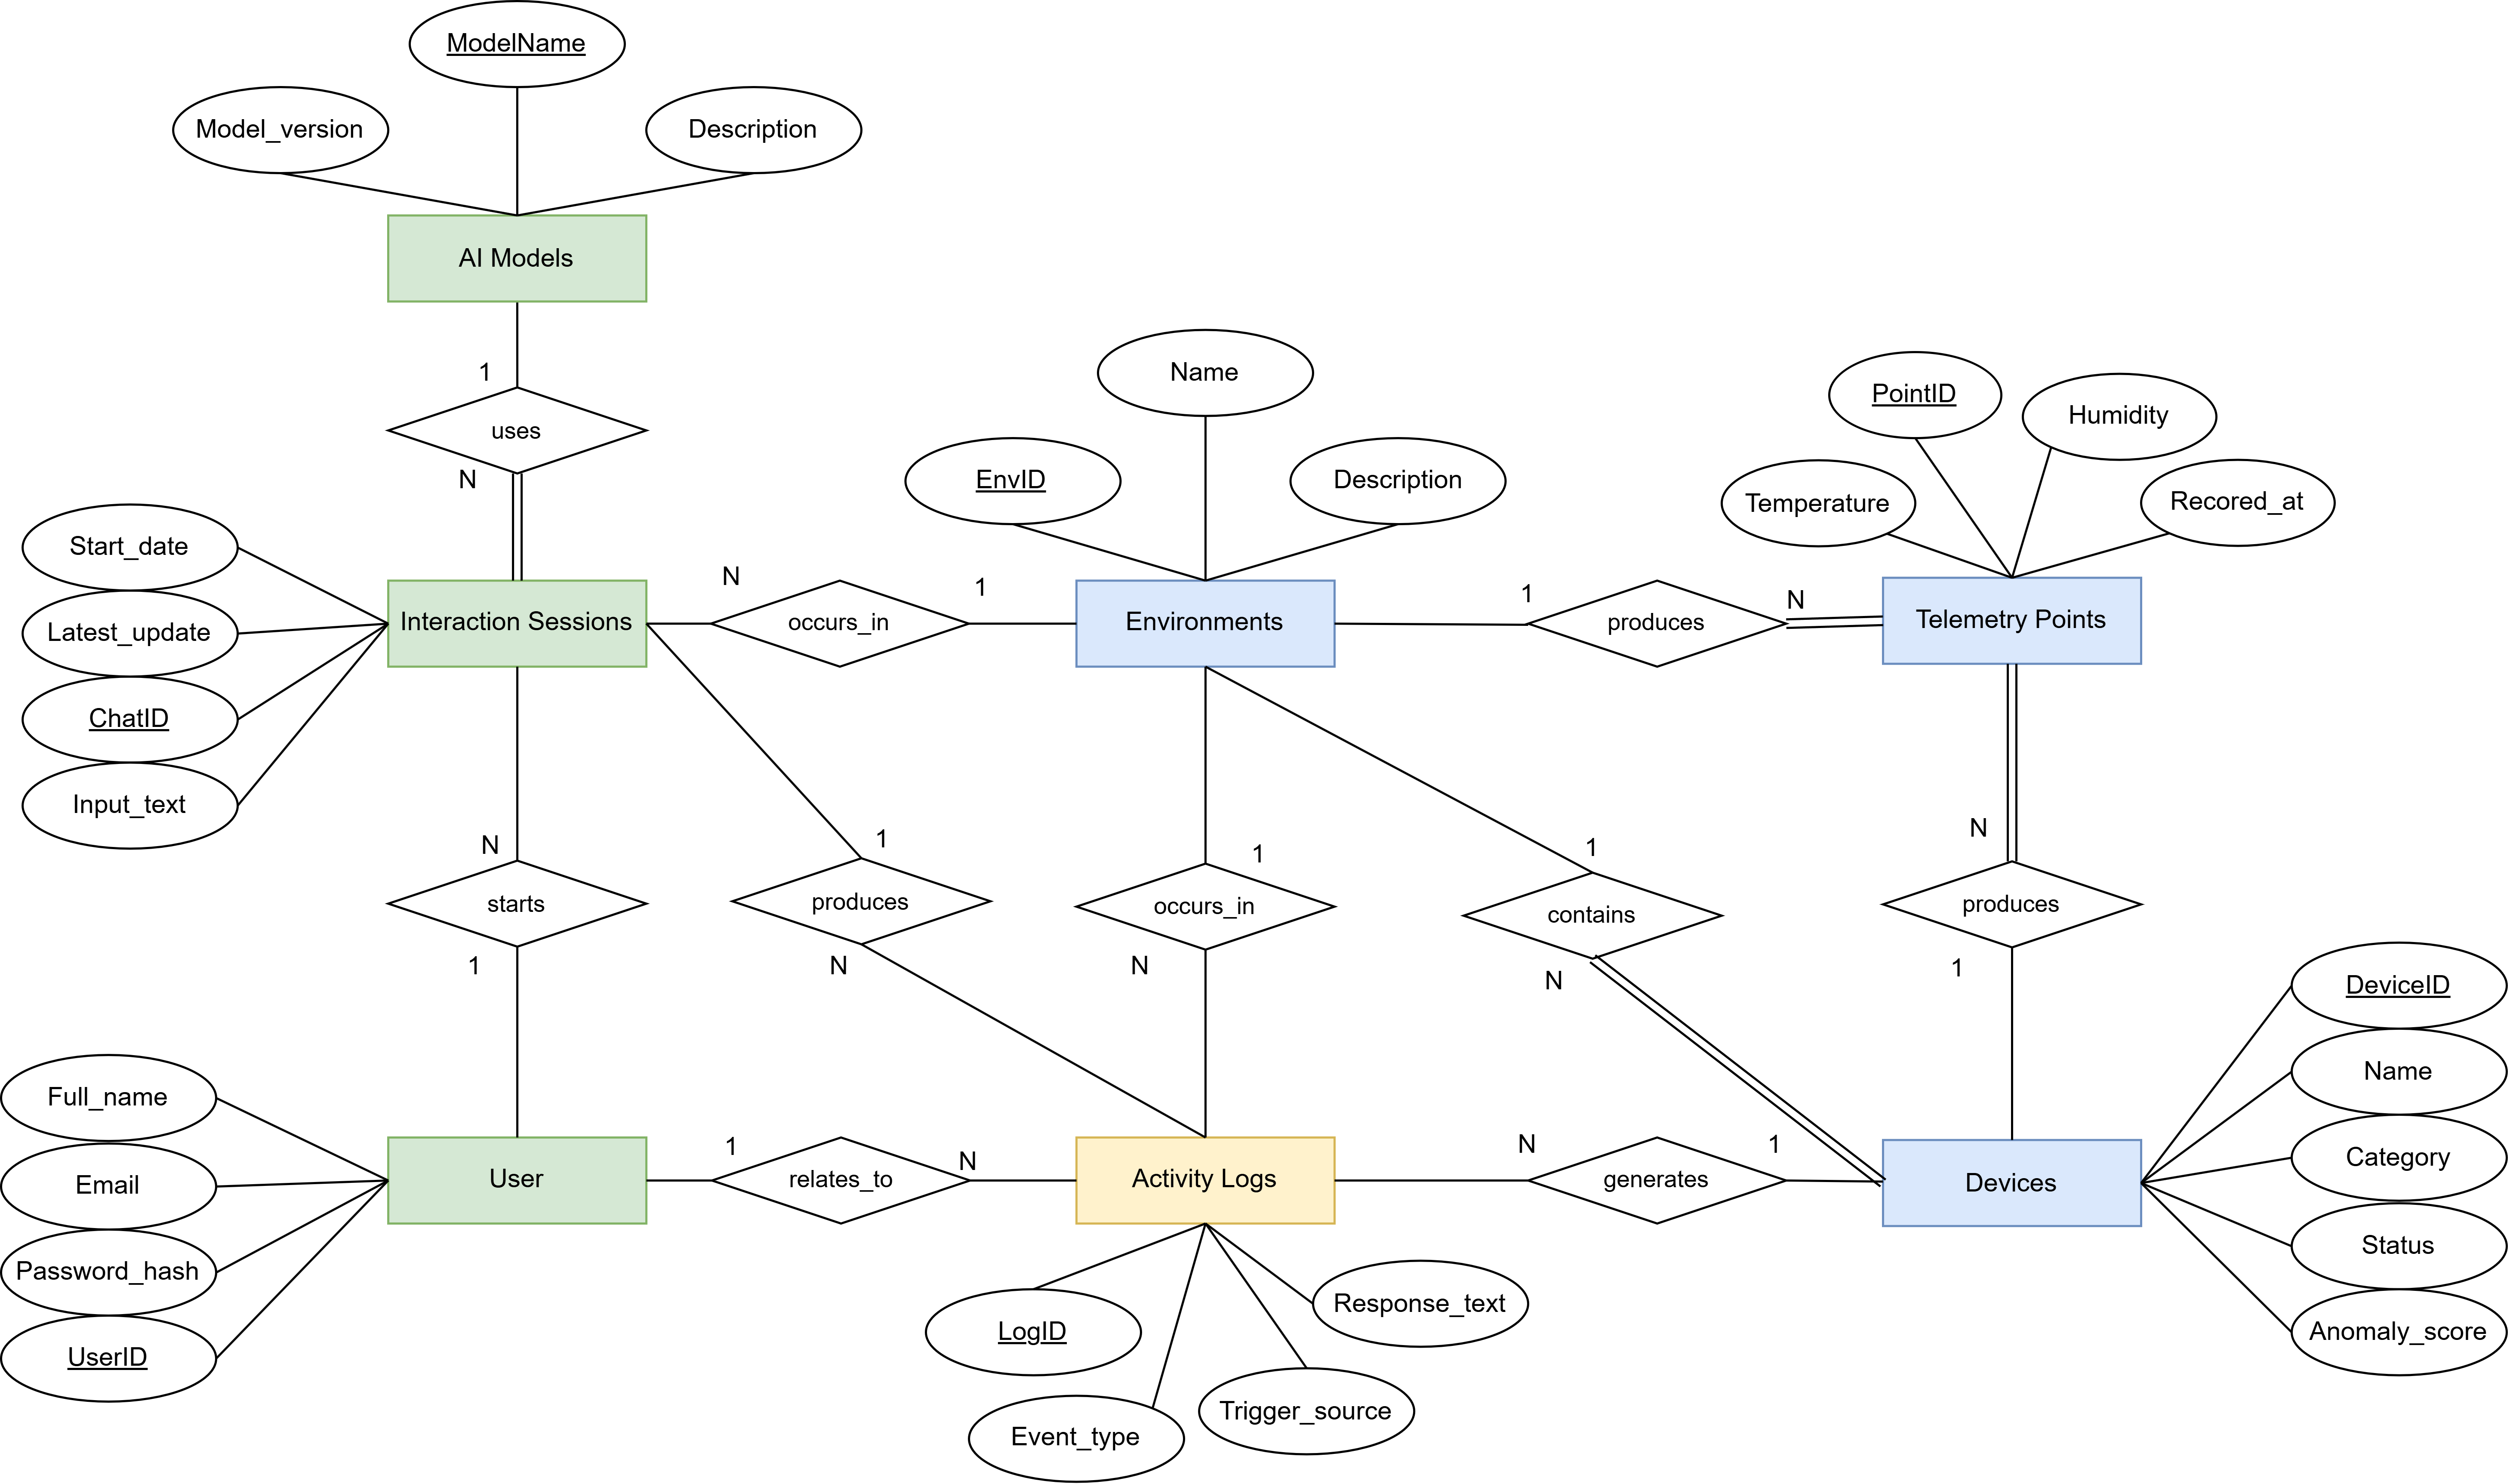
\includegraphics[width=0.95\textwidth]{image/EERD.png}
	\caption{EERD of H.E.R.A}
	\label{fig:EERD}
\end{figure}

\subsection{Relational Mapping}

\begin{figure}[H]
	\centering
	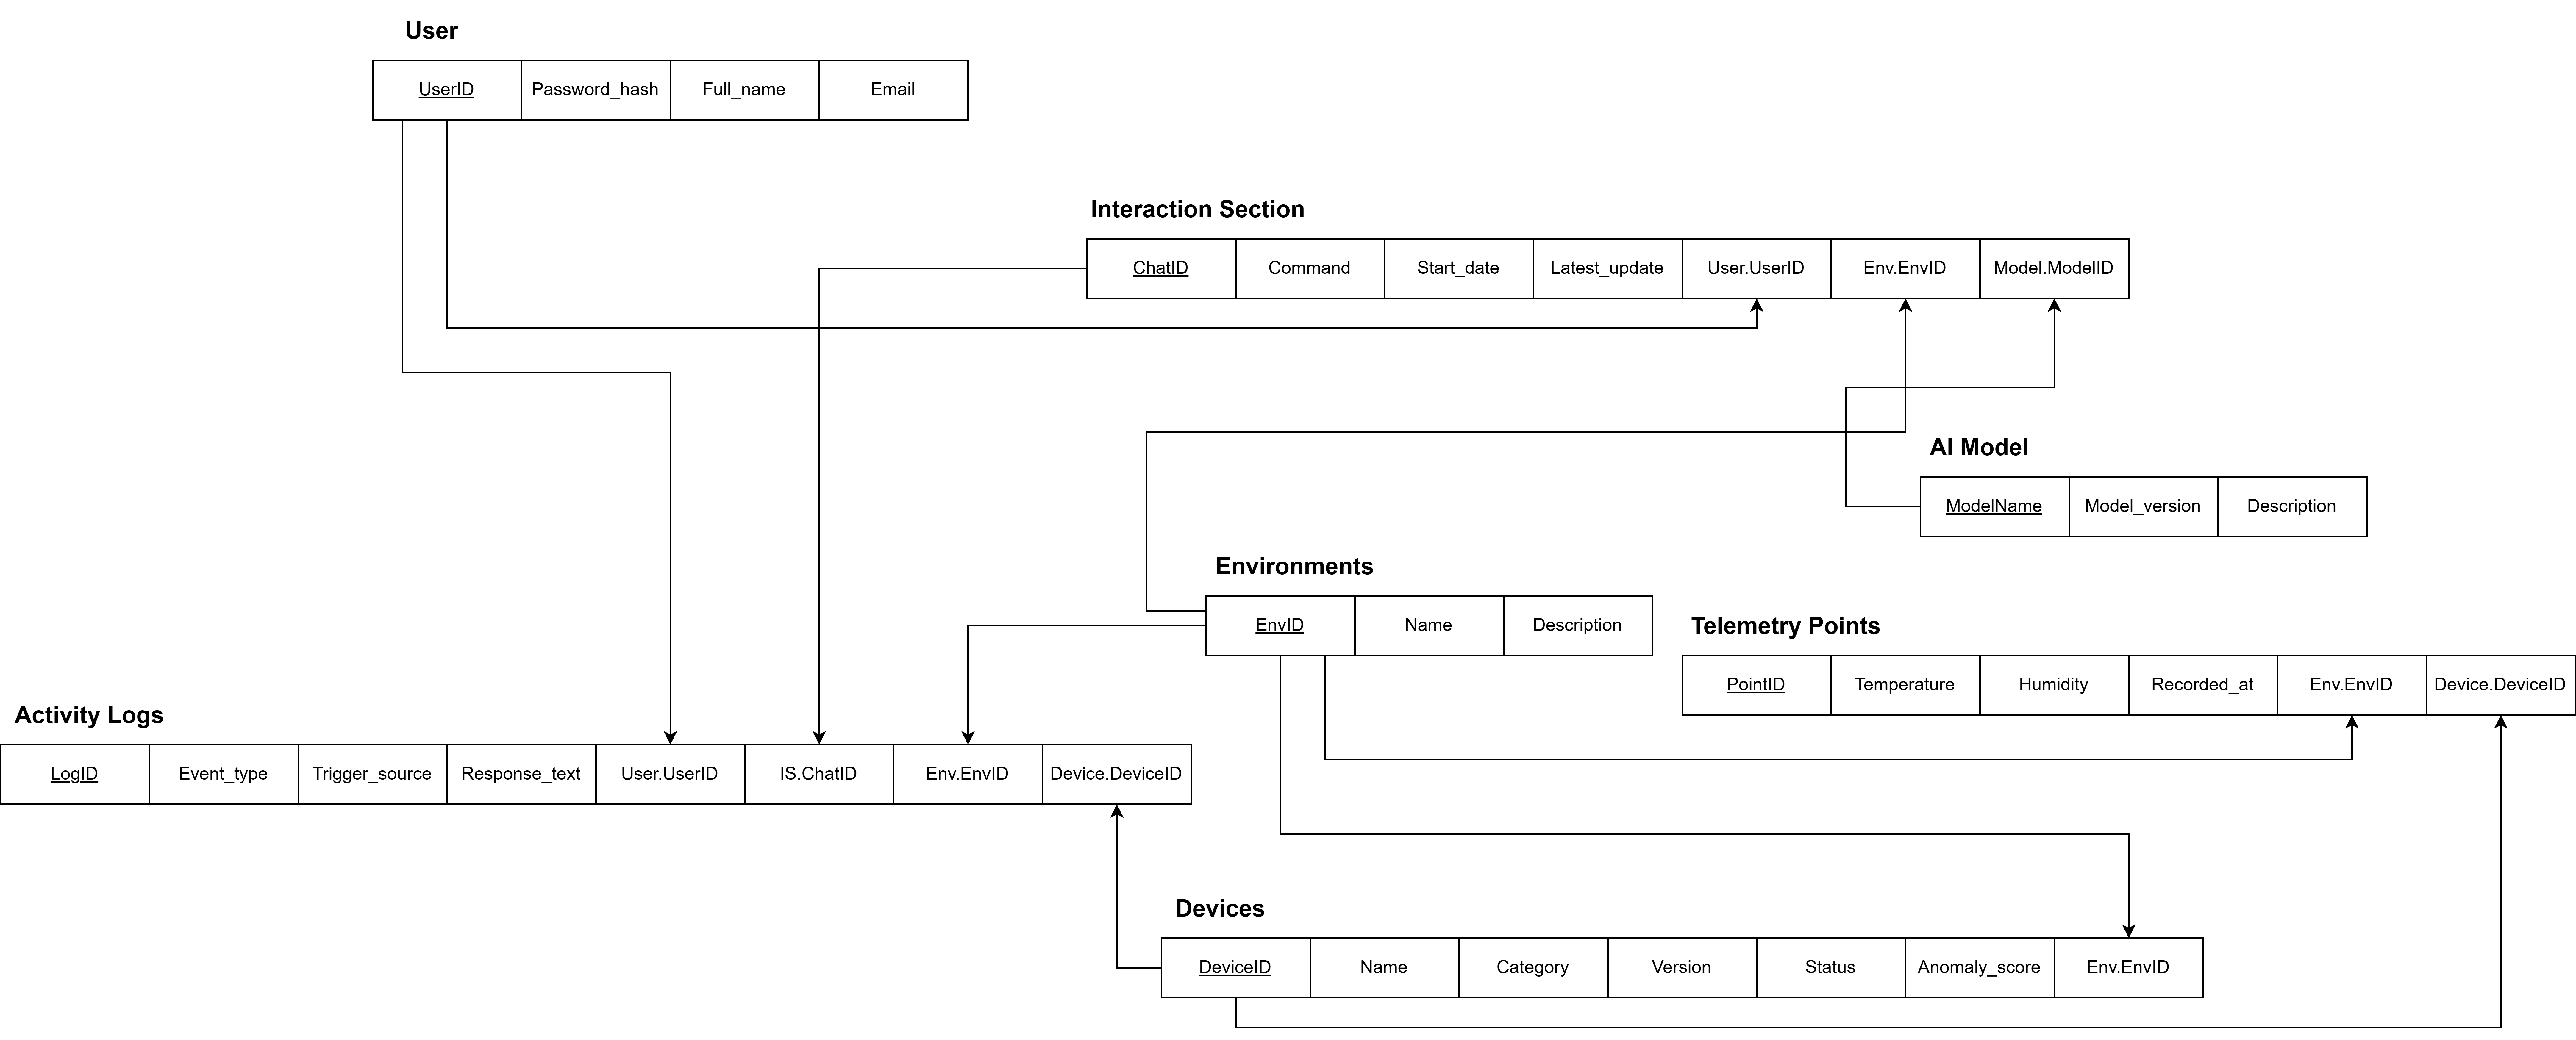
\includegraphics[width=0.90\textwidth]{image/RL.png}
	\caption{Relational Mapping of H.E.R.A}
	\label{fig:RL}
\end{figure}